% Created by tikzDevice version 0.12 on 2019-04-30 20:46:52
% !TEX encoding = UTF-8 Unicode
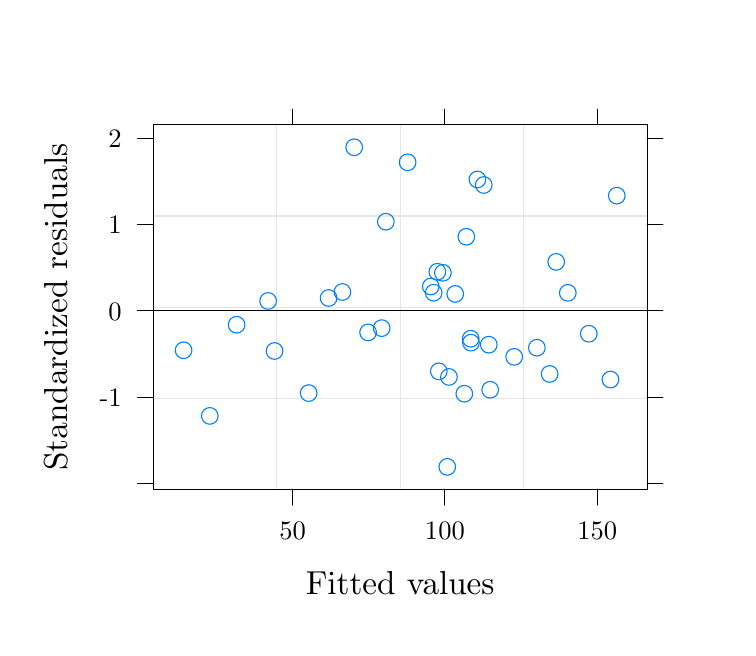
\begin{tikzpicture}[x=1pt,y=1pt]
\definecolor{fillColor}{RGB}{255,255,255}
\path[use as bounding box,fill=fillColor,fill opacity=0.00] (0,0) rectangle (252.94,216.81);
\begin{scope}
\path[clip] (  0.00,  0.00) rectangle (252.94,216.81);

\path[] (  0.00,  0.00) rectangle (252.94,216.81);
\definecolor{drawColor}{RGB}{0,0,0}

\node[text=drawColor,anchor=base,inner sep=0pt, outer sep=0pt, scale=  1.20] at (134.60, 12.05) {Fitted values};
\end{scope}
\begin{scope}
\path[clip] (  0.00,  0.00) rectangle (252.94,216.81);
\definecolor{drawColor}{RGB}{0,0,0}

\node[text=drawColor,rotate= 90.00,anchor=base,inner sep=0pt, outer sep=0pt, scale=  1.20] at ( 14.29,115.84) {Standardized residuals};
\end{scope}
\begin{scope}
\path[clip] (  0.00,  0.00) rectangle (252.94,216.81);
\definecolor{drawColor}{RGB}{0,0,0}

\path[draw=drawColor,line width= 0.4pt,line join=round,line cap=round] ( 95.74,181.67) -- ( 95.74,187.36);

\path[draw=drawColor,line width= 0.4pt,line join=round,line cap=round] (150.77,181.67) -- (150.77,187.36);

\path[draw=drawColor,line width= 0.4pt,line join=round,line cap=round] (205.81,181.67) -- (205.81,187.36);
\end{scope}
\begin{scope}
\path[clip] (  0.00,  0.00) rectangle (252.94,216.81);
\definecolor{drawColor}{RGB}{0,0,0}

\path[draw=drawColor,line width= 0.4pt,line join=round,line cap=round] ( 45.38, 52.14) -- ( 39.69, 52.14);

\path[draw=drawColor,line width= 0.4pt,line join=round,line cap=round] ( 45.38, 83.30) -- ( 39.69, 83.30);

\path[draw=drawColor,line width= 0.4pt,line join=round,line cap=round] ( 45.38,114.46) -- ( 39.69,114.46);

\path[draw=drawColor,line width= 0.4pt,line join=round,line cap=round] ( 45.38,145.62) -- ( 39.69,145.62);

\path[draw=drawColor,line width= 0.4pt,line join=round,line cap=round] ( 45.38,176.78) -- ( 39.69,176.78);

\node[text=drawColor,anchor=base east,inner sep=0pt, outer sep=0pt, scale=  0.96] at ( 34.00, 79.99) {-1};

\node[text=drawColor,anchor=base east,inner sep=0pt, outer sep=0pt, scale=  0.96] at ( 34.00,111.16) {0};

\node[text=drawColor,anchor=base east,inner sep=0pt, outer sep=0pt, scale=  0.96] at ( 34.00,142.32) {1};

\node[text=drawColor,anchor=base east,inner sep=0pt, outer sep=0pt, scale=  0.96] at ( 34.00,173.48) {2};
\end{scope}
\begin{scope}
\path[clip] (  0.00,  0.00) rectangle (252.94,216.81);
\definecolor{drawColor}{RGB}{0,0,0}

\path[draw=drawColor,line width= 0.4pt,line join=round,line cap=round] ( 95.74, 50.02) -- ( 95.74, 44.32);

\path[draw=drawColor,line width= 0.4pt,line join=round,line cap=round] (150.77, 50.02) -- (150.77, 44.32);

\path[draw=drawColor,line width= 0.4pt,line join=round,line cap=round] (205.81, 50.02) -- (205.81, 44.32);

\node[text=drawColor,anchor=base,inner sep=0pt, outer sep=0pt, scale=  0.96] at ( 95.74, 32.02) {50};

\node[text=drawColor,anchor=base,inner sep=0pt, outer sep=0pt, scale=  0.96] at (150.77, 32.02) {100};

\node[text=drawColor,anchor=base,inner sep=0pt, outer sep=0pt, scale=  0.96] at (205.81, 32.02) {150};

\path[draw=drawColor,line width= 0.4pt,line join=round,line cap=round] (223.83, 52.14) -- (229.52, 52.14);

\path[draw=drawColor,line width= 0.4pt,line join=round,line cap=round] (223.83, 83.30) -- (229.52, 83.30);

\path[draw=drawColor,line width= 0.4pt,line join=round,line cap=round] (223.83,114.46) -- (229.52,114.46);

\path[draw=drawColor,line width= 0.4pt,line join=round,line cap=round] (223.83,145.62) -- (229.52,145.62);

\path[draw=drawColor,line width= 0.4pt,line join=round,line cap=round] (223.83,176.78) -- (229.52,176.78);
\end{scope}
\begin{scope}
\path[clip] ( 45.38, 50.02) rectangle (223.83,181.67);
\definecolor{drawColor}{RGB}{230,230,230}

\path[draw=drawColor,line width= 0.4pt,line join=round,line cap=round] ( 45.38, 82.93) -- (223.83, 82.93);

\path[draw=drawColor,line width= 0.4pt,line join=round,line cap=round] ( 45.38,115.84) -- (223.83,115.84);

\path[draw=drawColor,line width= 0.4pt,line join=round,line cap=round] ( 45.38,148.76) -- (223.83,148.76);

\path[draw=drawColor,line width= 0.4pt,line join=round,line cap=round] ( 89.99, 50.02) -- ( 89.99,181.67);

\path[draw=drawColor,line width= 0.4pt,line join=round,line cap=round] (134.60, 50.02) -- (134.60,181.67);

\path[draw=drawColor,line width= 0.4pt,line join=round,line cap=round] (179.22, 50.02) -- (179.22,181.67);
\definecolor{drawColor}{RGB}{0,128,255}

\path[draw=drawColor,line width= 0.4pt,line join=round,line cap=round] ( 56.34,100.25) circle (  3.01);

\path[draw=drawColor,line width= 0.4pt,line join=round,line cap=round] (154.50,120.60) circle (  3.01);

\path[draw=drawColor,line width= 0.4pt,line join=round,line cap=round] (160.17,103.00) circle (  3.01);

\path[draw=drawColor,line width= 0.4pt,line join=round,line cap=round] ( 65.80, 76.52) circle (  3.01);

\path[draw=drawColor,line width= 0.4pt,line join=round,line cap=round] (108.74,119.13) circle (  3.01);

\path[draw=drawColor,line width= 0.4pt,line join=round,line cap=round] ( 86.88,118.05) circle (  3.01);

\path[draw=drawColor,line width= 0.4pt,line join=round,line cap=round] (123.01,106.69) circle (  3.01);

\path[draw=drawColor,line width= 0.4pt,line join=round,line cap=round] (101.54, 84.77) circle (  3.01);

\path[draw=drawColor,line width= 0.4pt,line join=round,line cap=round] (150.04,128.23) circle (  3.01);

\path[draw=drawColor,line width= 0.4pt,line join=round,line cap=round] (151.61, 58.10) circle (  3.01);

\path[draw=drawColor,line width= 0.4pt,line join=round,line cap=round] (212.87,156.10) circle (  3.01);

\path[draw=drawColor,line width= 0.4pt,line join=round,line cap=round] (117.98,173.59) circle (  3.01);

\path[draw=drawColor,line width= 0.4pt,line join=round,line cap=round] (127.93,108.24) circle (  3.01);

\path[draw=drawColor,line width= 0.4pt,line join=round,line cap=round] (157.78, 84.54) circle (  3.01);

\path[draw=drawColor,line width= 0.4pt,line join=round,line cap=round] ( 89.21, 99.98) circle (  3.01);

\path[draw=drawColor,line width= 0.4pt,line join=round,line cap=round] (162.52,161.96) circle (  3.01);

\path[draw=drawColor,line width= 0.4pt,line join=round,line cap=round] (183.99,101.15) circle (  3.01);

\path[draw=drawColor,line width= 0.4pt,line join=round,line cap=round] (190.98,132.17) circle (  3.01);

\path[draw=drawColor,line width= 0.4pt,line join=round,line cap=round] (148.04,128.59) circle (  3.01);

\path[draw=drawColor,line width= 0.4pt,line join=round,line cap=round] (148.57, 92.62) circle (  3.01);

\path[draw=drawColor,line width= 0.4pt,line join=round,line cap=round] (175.79, 97.86) circle (  3.01);

\path[draw=drawColor,line width= 0.4pt,line join=round,line cap=round] (146.72,121.04) circle (  3.01);

\path[draw=drawColor,line width= 0.4pt,line join=round,line cap=round] (188.61, 91.68) circle (  3.01);

\path[draw=drawColor,line width= 0.4pt,line join=round,line cap=round] (137.29,168.17) circle (  3.01);

\path[draw=drawColor,line width= 0.4pt,line join=round,line cap=round] (166.62,102.26) circle (  3.01);

\path[draw=drawColor,line width= 0.4pt,line join=round,line cap=round] (202.75,106.21) circle (  3.01);

\path[draw=drawColor,line width= 0.4pt,line join=round,line cap=round] (152.23, 90.60) circle (  3.01);

\path[draw=drawColor,line width= 0.4pt,line join=round,line cap=round] (164.80,159.96) circle (  3.01);

\path[draw=drawColor,line width= 0.4pt,line join=round,line cap=round] (195.17,120.99) circle (  3.01);

\path[draw=drawColor,line width= 0.4pt,line join=round,line cap=round] (160.08,104.41) circle (  3.01);

\path[draw=drawColor,line width= 0.4pt,line join=round,line cap=round] (158.51,141.26) circle (  3.01);

\path[draw=drawColor,line width= 0.4pt,line join=round,line cap=round] (167.13, 85.97) circle (  3.01);

\path[draw=drawColor,line width= 0.4pt,line join=round,line cap=round] ( 75.50,109.46) circle (  3.01);

\path[draw=drawColor,line width= 0.4pt,line join=round,line cap=round] (113.72,121.30) circle (  3.01);

\path[draw=drawColor,line width= 0.4pt,line join=round,line cap=round] (145.66,123.28) circle (  3.01);

\path[draw=drawColor,line width= 0.4pt,line join=round,line cap=round] (210.59, 89.66) circle (  3.01);

\path[draw=drawColor,line width= 0.4pt,line join=round,line cap=round] (129.43,146.70) circle (  3.01);
\definecolor{drawColor}{RGB}{0,0,0}

\path[draw=drawColor,line width= 0.4pt,line join=round,line cap=round] ( 45.38,114.46) -- (223.83,114.46);
\end{scope}
\begin{scope}
\path[clip] (  0.00,  0.00) rectangle (252.94,216.81);
\definecolor{drawColor}{RGB}{0,0,0}

\path[draw=drawColor,line width= 0.4pt,line join=round,line cap=round] ( 45.38, 50.02) rectangle (223.83,181.67);
\end{scope}
\end{tikzpicture}
